\documentclass{standalone}

\usepackage[OT1]{fontenc}
\renewcommand*\familydefault{\sfdefault}
\usepackage{helvet,sfmath}
\usepackage{siunitx}

\usepackage{tikz}
\usetikzlibrary{arrows,calc,patterns}
% \usetikzlibrary{intersections, calc, arrows.meta}
\usepackage{tikz,tkz-euclide}\usepackage{tikz}
\usepackage{amsmath}


\begin{document}



\tikzset{every picture/.style={line width=0.75pt}} %set default line width to 0.75pt        

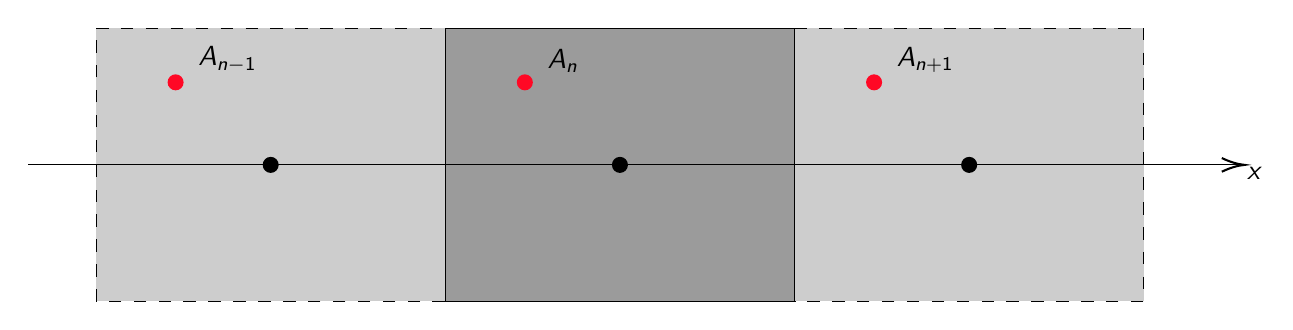
\begin{tikzpicture}[x=0.75pt,y=0.75pt,yscale=-1,xscale=1]
%uncomment if require: \path (0,6336); %set diagram left start at 0, and has height of 6336

%Shape: Rectangle [id:dp5310820997302841] 
\draw  [fill={rgb, 255:red, 155; green, 155; blue, 155 }  ,fill opacity=0.5 ][dash pattern={on 4.5pt off 4.5pt}] (542.71,5405) -- (710.97,5405) -- (710.97,5536.55) -- (542.71,5536.55) -- cycle ;
%Shape: Rectangle [id:dp9023995014000119] 
\draw  [fill={rgb, 255:red, 155; green, 155; blue, 155 }  ,fill opacity=0.5 ][dash pattern={on 4.5pt off 4.5pt}] (206.18,5405) -- (374.45,5405) -- (374.45,5536.55) -- (206.18,5536.55) -- cycle ;
%Shape: Rectangle [id:dp2274170810357714] 
\draw  [fill={rgb, 255:red, 155; green, 155; blue, 155 }  ,fill opacity=1 ] (374.45,5405) -- (542.71,5405) -- (542.71,5536.55) -- (374.45,5536.55) -- cycle ;
%Straight Lines [id:da6079653313054111] 
\draw    (626.84,5470.77) -- (757.5,5470.77) ;
\draw [shift={(759.5,5470.77)}, rotate = 180] [color={rgb, 255:red, 0; green, 0; blue, 0 }  ][line width=0.75]    (10.93,-3.29) .. controls (6.95,-1.4) and (3.31,-0.3) .. (0,0) .. controls (3.31,0.3) and (6.95,1.4) .. (10.93,3.29)   ;
%Straight Lines [id:da16998035185697213] 
\draw    (290.32,5470.77) -- (458.58,5470.77) ;
\draw [shift={(458.58,5470.77)}, rotate = 0] [color={rgb, 255:red, 0; green, 0; blue, 0 }  ][fill={rgb, 255:red, 0; green, 0; blue, 0 }  ][line width=0.75]      (0, 0) circle [x radius= 3.35, y radius= 3.35]   ;
\draw [shift={(290.32,5470.77)}, rotate = 0] [color={rgb, 255:red, 0; green, 0; blue, 0 }  ][fill={rgb, 255:red, 0; green, 0; blue, 0 }  ][line width=0.75]      (0, 0) circle [x radius= 3.35, y radius= 3.35]   ;
%Straight Lines [id:da8384465289980407] 
\draw    (173.5,5470.77) -- (290.32,5470.77) ;
%Straight Lines [id:da6730275374056559] 
\draw    (458.58,5470.77) -- (626.84,5470.77) ;
\draw [shift={(626.84,5470.77)}, rotate = 0] [color={rgb, 255:red, 0; green, 0; blue, 0 }  ][fill={rgb, 255:red, 0; green, 0; blue, 0 }  ][line width=0.75]      (0, 0) circle [x radius= 3.35, y radius= 3.35]   ;
%Straight Lines [id:da3720880022120362] 
\draw [color={rgb, 255:red, 255; green, 8; blue, 37 }  ,draw opacity=1 ]   (244.5,5431) ;
\draw [shift={(244.5,5431)}, rotate = 0] [color={rgb, 255:red, 255; green, 8; blue, 37 }  ,draw opacity=1 ][fill={rgb, 255:red, 255; green, 8; blue, 37 }  ,fill opacity=1 ][line width=0.75]      (0, 0) circle [x radius= 3.35, y radius= 3.35]   ;
%Straight Lines [id:da9752434175126328] 
\draw [color={rgb, 255:red, 255; green, 8; blue, 37 }  ,draw opacity=1 ]   (412.76,5431) ;
\draw [shift={(412.76,5431)}, rotate = 0] [color={rgb, 255:red, 255; green, 8; blue, 37 }  ,draw opacity=1 ][fill={rgb, 255:red, 255; green, 8; blue, 37 }  ,fill opacity=1 ][line width=0.75]      (0, 0) circle [x radius= 3.35, y radius= 3.35]   ;
%Straight Lines [id:da37719196685879053] 
\draw [color={rgb, 255:red, 255; green, 8; blue, 37 }  ,draw opacity=1 ]   (581.03,5431) ;
\draw [shift={(581.03,5431)}, rotate = 0] [color={rgb, 255:red, 255; green, 8; blue, 37 }  ,draw opacity=1 ][fill={rgb, 255:red, 255; green, 8; blue, 37 }  ,fill opacity=1 ][line width=0.75]      (0, 0) circle [x radius= 3.35, y radius= 3.35]   ;

% Text Node
\draw (254.18,5427.55) node [anchor=south west] [inner sep=0.75pt]   [align=left] {$\displaystyle A_{n-1}$};
% Text Node
\draw (422.45,5427.55) node [anchor=south west] [inner sep=0.75pt]   [align=left] {$\displaystyle A_{n}$};
% Text Node
\draw (590.71,5427.55) node [anchor=south west] [inner sep=0.75pt] [align=left] {$\displaystyle A_{n+1}$};
% Text Node
\draw (759.5,5470.77) node [anchor=north west][inner sep=0.75pt]    {$x$};


\end{tikzpicture}
\end{document}